\documentclass[conference]{IEEEtran}
\IEEEoverridecommandlockouts
\usepackage{cite}
\usepackage{amsmath,amssymb,amsfonts}
\usepackage{algorithmic}
\usepackage{graphicx}
\usepackage{textcomp}
\usepackage{xcolor}

\def\BibTeX{{\rm B\kern-.05em{\sc i\kern-.025em b}\kern-.08em
    T\kern-.1667em\lower.7ex\hbox{E}\kern-.125emX}}
\usepackage{amssymb, graphicx, natbib}
\usepackage{fancyhdr, fontspec,bidipoem, polyglossia, multirow}
\setmainlanguage{english}   % main language for the document will be English use numerals=weastern if numbers in weastern style 
\setotherlanguage[numerals=weastern]{urdu}
\newfontfamily\urdufont[Script=Arabic,Scale=1.4]{Jameel Noori Nastaleeq}  % or Nafees or Scheherazade
%%
\def\BibTeX{{\rm B\kern-.05em{\sc i\kern-.025em b}\kern-.08em
    T\kern-.1667em\lower.7ex\hbox{E}\kern-.125emX}}

\begin{document}

\title{Neural Encoder-Decoder based Urdu Conversational Agent\\
}

\author{\IEEEauthorblockN{Mehreen Alam}
\IEEEauthorblockA{\textit{Department of Computer Science} \\
\textit{NUCES}\\
Islamabad, Pakistan \\
mehreen.alam@nu.edu.pk}
\and
\IEEEauthorblockN{Sibt ul Hussain}
\IEEEauthorblockA{\textit{Department of Computer Science} \\
\textit{NUCES}\\
Islamabad, Pakistan \\
sibtul.hussain@nu.edu.pk}
}

\maketitle

\begin{abstract}
Conversational agents have very much become part of our lives since the reuse of neural network based models for their development. Previously used manually annotated and rule based methods lacked the scalability and generality of the conversational agents. The neural conversational agent has two parts: at one end an encoder understands the question while the other  end decoder prepares and outputs the corresponding answer to the question asked. Both the parts are based on recurrent neural network and combined together in an end-to-end fashion. Conversational agents for Urdu language is an area where not much work has been done, especially recent state of the art neural network based techniques have not been explored yet. In this paper, we apply deep neural network based technique of encoder-decoder using attention mechanism to build an Urdu language based conversational agent - here we limit the knowledge base of our agent to general knowledge regarding Pakistan. Overall, this work makes following contributions: 1) we create a dataset of 5000 question-answer pairs; and 2) we present a new deep encoder-decoder based conversational agent for Urdu language. Our best model has the BLEU score of 58 and gives syntactically and semantically correct answers in majority of the cases.
\end{abstract}

\begin{IEEEkeywords}
deep learning, machine learning, conversational model, sequence to sequence, chatbot, Urdu language
\end{IEEEkeywords}

\section{Introduction}

Advances in end to end training of deep neural networks have led to huge successes in a variety of fields, automatic speech recognition, natural language processing and computer vision. One such area that has seen a significant leap in performance is the area of conversational modeling where humans put up a conversation with with a conversational agent in such a way that makes it hard for the humans to figure out if they are talking to a machine or another human. As conversing with a human is a very complex and complicated problem, it is usually addressed to with restrictions. One such restriction could be limiting the conversational model to a specific domain. Other could be answering only to the question posed and not keeping the whole context of previous or the coming (predicted) questions/answers in mind. Even after the addition of these restrictions, there is still a lot of work needed to be done to achieve human level performance.

In our work, we have chosen the domain of general knowledge of Pakistan and keep the context of one question-answer pair only. The language chosen is Urdu which is understood by at least 20 million people in the world. To date, to the best of our knowledge, there is no publicly available conversational model available for Urdu language in any domain for that matter. Nor was there any publicly available dataset in Urdu that could be used to build the conversational model. To address this research problem, we transformed our question answering problem to the deep learning technique of sequence to sequence proposed  by \cite{sutskever2014sequence} and also make the first ever question answering database in Urdu language in the domain of general knowledge of Pakistan. We make the following contributions:
 
\begin{enumerate}
\item Create a parallel corpus of 5000 question-answers pairs in Urdu language in the domain of general knowledge of Pakistan, and 
\item Design a model for the Urdu based conversational agent in the domain of general knowledge of Pakistan.
\end{enumerate}

The model we have used for our system is based on bi-directional encoder and attention based decoder. Bi-directional encoders learn in the forward as well as the backward direction, thereby increasing the learning capacity of the encoder \cite{BahdanauCB14}. Attention mechanisms show remarkable improvement in quality as they tend to focus on the relevant parts of the question while producing the answers \cite{BahdanauCB14}. We have used long short-term memory networks rather than vanilla recurrent neural network or its variations, since lstms overcome the problem of vanishing gradients and give better mapping even for longer questions and answers according to \cite{hochreiter1997long}. For our problem, single layer of encoder and decoder gave the most optimal results qualitatively and quantitatively. The evaluation metric used for judging the quality of answers generated for every question is the standard Bilingual Evaluation Understudy (BLEU) proposed by \cite{papineni2002bleu}. The aforementioned evaluation criteria is relevant to our model as we map questions asked as the input sequence while the answers are mapped onto the output sequence.   
   
The layout of the paper is as follows. We present background study and motivation in the next section. Section III throws light on the model architecture in detail, followed by the how we built the dataset in section IV. We give the details of our experimental settings in section V and a thorough discussion on the results of our model in section VI. We finally conclude our paper in section VII and highlight the future directions. 	

\section{Background Study and Motivation}

Humans use currently available textual conversational agents, like A.L.I.C.E. and Miksuku to help them in completing specific tasks or merely to put up a conversation. Work in this domain picked up pace with the introduction of increased compute power and deeper networks for enhanced learning. Conventional techniques are usually template-based or heuristic based as have been used by \cite{Nio2014,Ameixa2014}. Currently, data-driven end-to-end training using deep learning techniques is used by 
\cite{Serban2016building, Shang2015, Sordoni2015, Gao2018neural}. 

Since the problem is too diverse and complex, work has been done by looking at only a specific portion of the problem. \cite{chen2017survey} categorizes the problem into task-oriented and non-task oriented conversational agents. The former works as an assistant to the user for specific trained tasks like flight reservations, hotel booking. Non-task oriented systems are primarily built to converse with humans in a general way, chatbots is a common example. Major approaches used for building non-task oriented systems are: a) generative models which generate responses to the questions posed, and b) retrieval-based models that refer to a knowledge base before producing the answer. Generative models have the edge of conversing more human-like though the content may lack meaning. Retrieval based systems are more accurate but are more blunt and thus less likely to put up conversations closer to humans. Other ways of looking at the conversational modeling problem is either source to target mapping problem \cite{ritter2011data} or domain specific modeling problem \cite{banchs2012iris}. 
 
One of the modern ways of looking at the problem of conversational model is to map it onto a machine translation task \cite{ritter2011data}. After the introduction of sequence to sequence models by \cite{sutskever2014sequence}, many attempts have been made to extend the work by using this model \cite{Serban2016building, Sordoni2015, ritter2011data}. Variations to the encoder-decoder model are explored, for example, bi-directional encoder \cite{BahdanauCB14}, attention based decoder \cite{BahdanauCB14} and use of word embeddings \cite{mikolov2013distributed, pennington2014glove} to enrich the learning, to name a few. However, to date, no such attempt has been made using any of the state-of-the-art deep learning based technique to work in line with building a conversational model for Urdu language. Most prominent ones like \cite{kaleem2014development, arain2018artificial} are task-oriented and use conventional methods. This leaves a big research gap in the domain of conversational modeling while in the context of Urdu language no prior attempt has been made.

To the best of or knowledge, our work is the first effort in the direction of building an Urdu based conversational agent in the domain of general knowledge of Pakistan using deep learning based sequence to sequence networks.   

\section{Model and its Architecture}

We have used sequence to sequence model with bi-directional encoder and attention mechanism. Bi-directional encoder has the enhanced capacity as it learns in the forward as well as backward time direction. The attention mechanism spreads the learnt embedding for a question to a series of annotation vectors which at every step of generating the answer brings the focus to the relevant words in the question. This approach overcomes the bottleneck of relying on just one context vector where the question was embedded.

Specifically, our model has two RNNs: encoder and decoder. Encoder embeds the question of $n$ words, $x_1,x_2,...,x_n$, into a series of context vectors, \textbf{$c_1, c_2,...,c_n,$}, while the decoder uses this vector to predict the answer of $m$ words, $y_1, y_2, ..., y_m$.  This is done by using the conditional probability, $p(y|x)$, such that question statement, \textbf{$x$}, has the answer statement, \textbf{$y$} and is explained in \ref{eq:1}.	 

\begin{equation}\label{eq:1}
\log p(y|x) = \sum_{j=1}^{m} \log p (y_j|y_{<j},c_j) 
\end{equation}
such that   
\begin{equation}\label{eq:2}
p (y_j|y_{<j},c_j) = softmax (w(h_j)) 
\end{equation}
where probability of every word to be predicted, $y_j$, given the previous words predicted, $y_{<j}$ and the context vector, $c_j$, is equal to taking softmax over $w$, which is the transformation function that maps onto the vector of the size of vocabulary and $h_j$ is the LSTM output in the decoder network which is computed as 

\begin{equation}\label{eq:3}
h_{j} = concat[f (x_j,{h}_{j-1});f (x_j,{h}_{j+1})] 
\end{equation}

These annotations are used to find context vector, $c_j$, for every output word, $y_j$, such that 

\begin{equation}\label{eq:6}
c_{j} = \sum_{j=1}^{n} \alpha_{ji}h_i 
\end{equation}
where the weight, $\alpha_{ji}$, for each annotation vector, $h_i$, is:

\begin{equation}\label{eq:7}
\alpha_{ji} = \exp(g_{ji})/\sum_{k=1}^{n} \exp (g_{jk}) 
\end{equation}

\begin{figure}[h!]
  \centering
    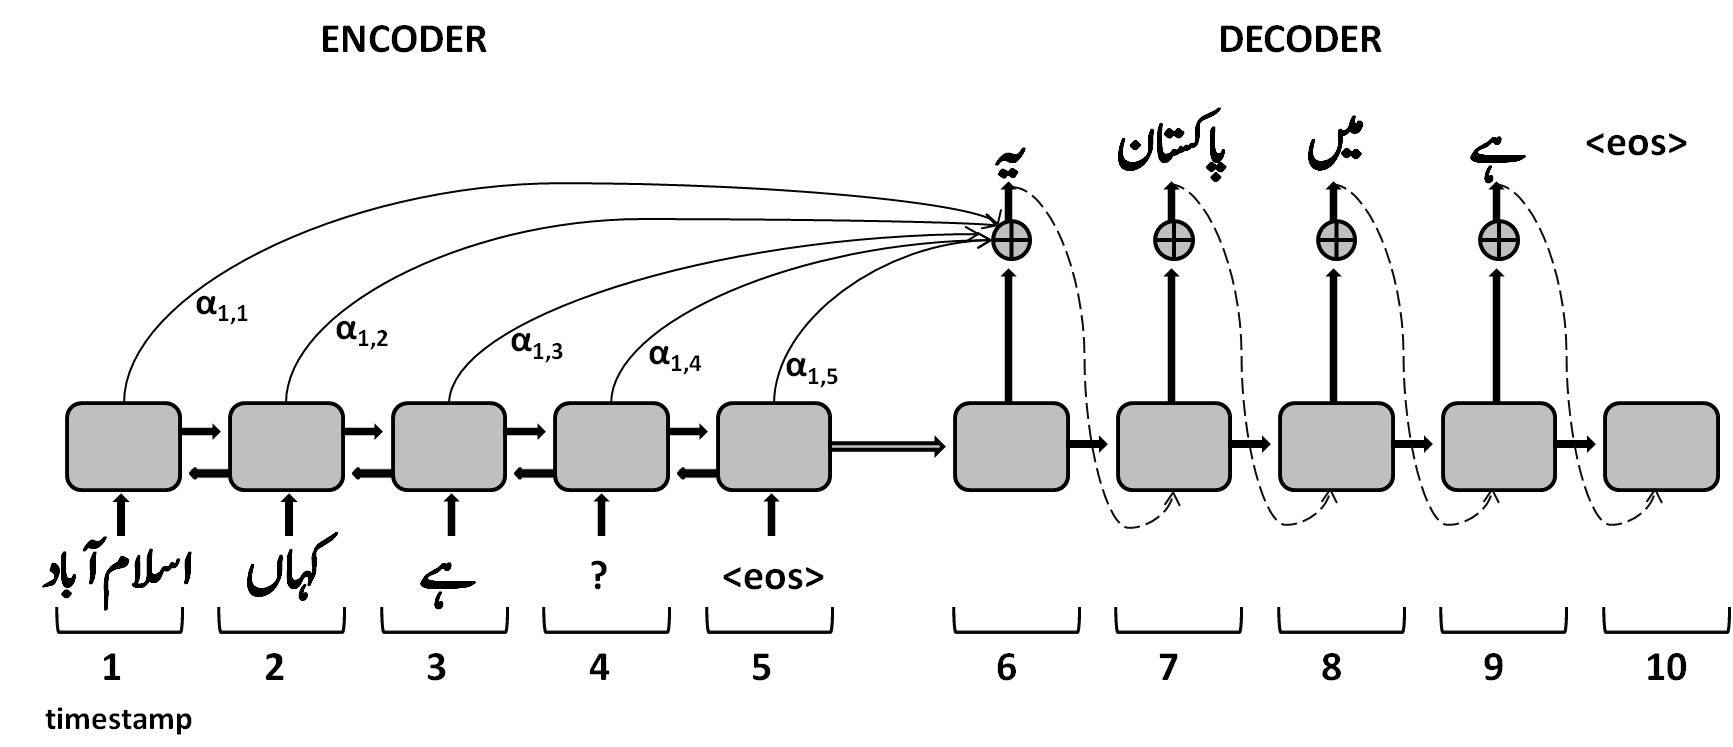
\includegraphics[width=\linewidth]{Attention-Bi-directional-Encoder-Decoder.png}
  \caption{An example of how question-answer pair is mapped to bi-directional encoder and attention based decoder. We show context vector for the first word of the answer sequence.}
  \label{fig:attention-model}
\end{figure}

The context vector, $c_{j}$, for ever output word is used by the decoder to focus on only the relevant words from the input question. Instead of a single generic context vector, a distributed context vector improves the answering capability. Specifically, each of these annotation vectors convey to the model the extent to which every word in the question is related to the current output answer work. $g_{ji}$ is calculated from the annotation vector, $h_{i}$, and $s_{j-1}$, which is the output of the LSTM hidden unit just before emitting $y_j$.
 
\section{Dataset}
As deep learning techniques are data-driven, good output quality heavily depends upon availability of a good dataset. Absence of any publicly available question answering data set, regardless of the domain, is the main reason for any progress done in this research direction. So, we had to build the dataset from scratch. 

For us, it was a challenging task as there is no crowd sourcing facility available for Urdu language. The very famous Amazon Mechanical Turk is not operative in Pakistan. So, we came up with the novel idea of collecting data from 300 students of our university who entered questions into our database via a web portal we designed especially for this crowd sourcing facility. We gave them a list of topics in the context of Pakistan from which they could ask questions, for example about rivers, presidents, education, sports, provinces and economy, to name a few. This helped us capture the inherent diversity of the type and the way questions can be posed. This way we were able to get over 5000 general knowledge questions about Pakistan. Since the main part of a conversational agent is to understand the intent of the question which when found is mapped to one specific answer. To reach a wider audience, multiple questions and corresponding answer have been mentioned in english language, while originally everything was done completely in Urdu. For example, the answer for all the questions mentioned below is  \textquotedblleft
Imran Khan\textquotedblright:

\begin{enumerate}
\item Who is the Prime Minister of Pakistan?
\item Who is the Prime Minister? 
\item Who is the current Prime Minister of Pakistan?
\item Prime Minister?
\item Prime Minister of Pakistan?
\end{enumerate}

Data pre-processing step was intense as it needed manual as well as algorithmic techniques to remove the irrelevant questions and to fix the irregularities found in any question. It is worth mentioning that we did not fix the human errors as in real life humans are prone to enter questions such that may have grammatical or spelling errors but do make a sense overall. As an example, we list four versions of the question where each version has either a grammatical or a spelling mistake. All variations like these are part of our dataset. We have underlined the misspelled or incorrect words entered in the following examples:

\begin{itemize}
\item \RL{\begin{urdu} پاکستان کا وزیر اعظم کون  \underline{ حے}؟  \end{urdu}}
\item \RL{\begin{urdu} پاکستان کا وزیر اعظم \underline{ کیا} ہے ؟  \end{urdu}}
\item \RL{\begin{urdu} پاکستان کا وزیر اعظم \underline{ کب} ہے ؟  \end{urdu}}
\item \RL{\begin{urdu} پاکستان کا \underline{ وزیر اعضم }کون ہے ؟  \end{urdu}}
\end{itemize}

This way we were able to capture the irregularities from a big majority of people which helped us make our model generic, scalable and focused in guessing the intent of the question while ignoring minor spelling or grammatical mistakes. After cleaning the data, we manually entered relevant answers to every question. Additionally, our model is independent of the sequence length which means it does not require the sequence lengths of the question and the corresponding answer be the same. This further makes our model more flexible and better prepared to understand the real-life diversities inherent in the language.

\section{Experimental Settings}
Thorough experimentation was done on GPU machines to find the most optimal parameters and hyper-parameters for the model. Cross validation was also done to make sure the model does not over-fit and gives us the most generic output. One layer deep LSTMs were chosen for both the encoder and the decoder after trying layer depths of 1,2,3,4 and 5. Hidden units in lstms, attention head and embedding dimension were all set to 128 after trying randomly between 64 to 2048 neurons all combinations in powers of 2. The sequence length was restricted to 30 with three buckets (0-10, 10-20, 20>). Adam was used the optimizer with learning rate of 0.0001 initially and 0.001 once the model had matured. Attention mechanism is used and encoders are used with bi-directional option. Our data was randomly shuffled and divided into train, validation and test set in the ratio of 3:1:1.

\section{Results and Discussions}

\subsection{Quantitative Analysis}
After thorough experimentation and cross validation on the dataset created by us, our final model is the one presented earlier in Section III. It gave us the maximum BLEU score of 62 and minimum cross entropy loss of 0.5 on the validation dataset as seen from figure \ref{fig:bleu-score} and figure \ref{fig:loss}, outperforming any other combination of the network and its parameters within the time constraints. Thus, the model trained at 18K is the most optimal, we save that model and run it on the test set where it gives us the BLEU score of 58. 
 
\begin{figure}[h!]
  \centering
    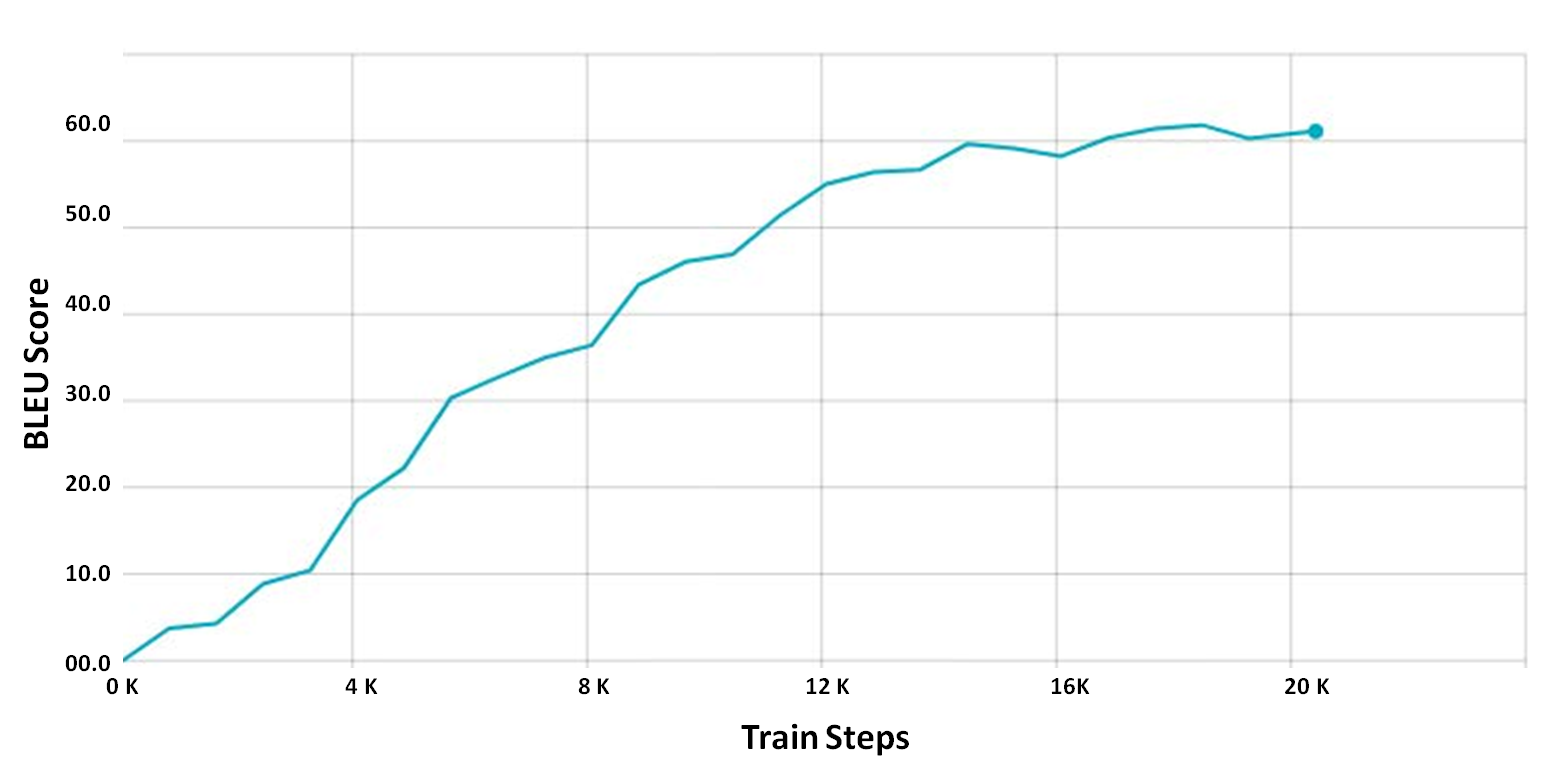
\includegraphics[width=\linewidth]{bleu-score.png}
  \caption{Bleu Score on Validation Dataset on a total of 25 K train steps. As can be seen that the model gives the top BLEU score of 62 at around 18K train steps.}
  \label{fig:bleu-score}
\end{figure}

\begin{figure}[h!]
  \centering
    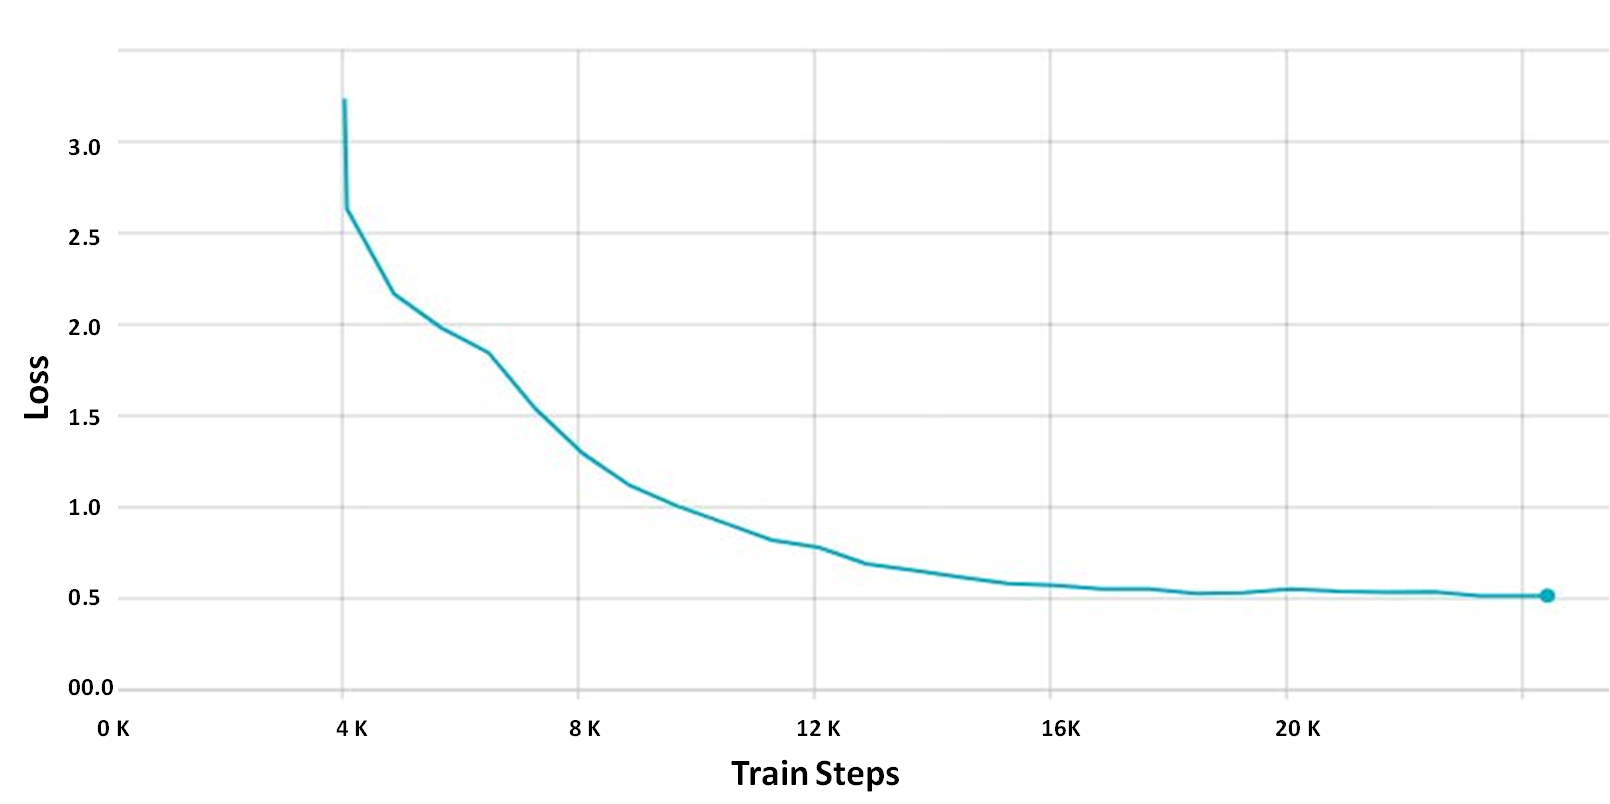
\includegraphics[width=\linewidth]{loss.png}
  \caption{Loss on Validation Dataset on a total of 25 K train steps. In line with the BLEU score seen in figure above, the model has the lowest loss around 18K train steps.}
  \label{fig:loss}
\end{figure}


\subsection{Qualitative Analysis}

A BELU score of 58 achieved by the model is a strong indication that the model is generic and generates accurate responses for majority of the cases. Table \ref{table:correct-answers} shows the result. It can be observed from the examples in the table that the model digs the intent of the question even when question has an ambiguity. For example, the first question in table \ref{table:correct-answers} which is asked differently than the regular way, our model has still grasped the intent of the question and answers exactly as a human shall do. Any question for which the model is not able to generate the relevant answer with a high probability, it refers to a one of the default answers requesting more clarity in posing the question as evident from question 7. Overall, it is very encouraging to observe that all answers are not only syntactically and  grammatically correct but are also relevant and conceptually meaningful.   

\begin{table}[]
\centering
\caption{Completely correct answers for the questions asked to our conversational agent}
\label{table:correct-answers}
\begin{tabular}{|r|r|r|}
\hline
Answers                                                                 & Questions              &No.\\ \hline
\RL{\begin{urdu}.اسلام آباد پاکستان کا دارالحکومت ہے \end{urdu}}                                    & \RL{\begin{urdu}اسلام آباد کیا ہے؟ \end{urdu}}    &1\\ \hline
\RL{\begin{urdu}.اسلام مذہب ہے  \end{urdu}}                                                         & \RL{\begin{urdu}اسلام کیا ہے؟ \end{urdu}}         &2\\ \hline
\RL{\begin{urdu}.جیسمین پاکستان کا قومی پھول ہے \end{urdu}}                                         & \RL{\begin{urdu}پاکستان کا قومی پھول؟ \end{urdu}} &3\\ \hline
\RL{\begin{urdu}.یہ پاکستان میں ہے  \end{urdu}}                                                     & \RL{\begin{urdu}اسلام آباد کہاں ہے؟ \end{urdu}}   &4\\ \hline
\RL{\begin{urdu}.میرے دوست ہو جو پاکستان کے بارے میں معلومات چاہتے ہو \end{urdu}} & \RL{\begin{urdu} میں کون ہوں؟  \end{urdu}}         &5\\ \hline
\RL{\begin{urdu}.میں ایک بوٹ ہوں  \end{urdu}}                                                       & \RL{\begin{urdu}تم کون ہو؟ \end{urdu}}            &6\\ \hline
\RL{\begin{urdu}.کسی بھی الجھن سے بچنے کے لئے، براہ کرم مزید مخصوص رہیں \end{urdu}}                 & \RL{\begin{urdu}پاکستان کا دارالحکومت؟ \end{urdu}} &7\\ \hline
\end{tabular}
\end{table}

However, our model does makes mistakes on rare occasions. For analysis purposes, we have categorized the mistakes the model makes in two main ways: 1) conceptual, and 2) grammatical.  Since deep learning techniques are data-driven, any question asked from a context the model has not seen before leads to an answer which may be conceptually irrelevant to the question asked but may be completely correct sentence otherwise, refer table \ref{table:incorrect-answers} question no 3. Rest of the questions have been answered in conceptually correct manner with an error or two in appropriate preposition selection as highlighted by underlining the words. 

\begin{table}[]
\centering
\caption{Answers having mistakes for the questions asked to our conversational agent}
\label{table:incorrect-answers}
\begin{tabular}{|r|r|r|}
\hline
Answers                                                                                    & Questions                  &No.\\ \hline
\RL{\begin{urdu} قائد اعظم پاکستان \underline{ کا }بانی \underline{ .ہے } \end{urdu}}& \RL{\begin{urdu}پاکستان کا بانی کون ہے؟     \end{urdu}}  &1\\ \hline
\RL{\begin{urdu} آم پاکستان \underline{ کے }.قومی پھل ہے  \end{urdu}}                                  & \RL{\begin{urdu}پاکستان کا قومی پھل کیا ہے؟ \end{urdu}} &2\\ \hline
\RL{\begin{urdu} \underline{ .یہ پاکستان کا قومی پھول ہے}   \end{urdu}}                                & \RL{\begin{urdu}کس نے ورلڈ کپ جیتا؟        \end{urdu}} &3\\ \hline
\RL{\begin{urdu} ممنون  حسین پاکستان \underline{ کا }صدر \underline{ .ہے }\end{urdu}} & \RL{\begin{urdu}ممنون حسین کون ہے؟        \end{urdu}}  &4\\ \hline
\RL{\begin{urdu} \underline{ .پنجاب میں دارالحکومت ہے } \end{urdu}}                                    & \RL{\begin{urdu}پنجاب کہاں واقع ہے ؟    \end{urdu}} &5\\ \hline   
\end{tabular}
\end{table}

\section{Conclusions}
It was motivating to see that the first ever attempt to make an Urdu conversational agent in the domain of general knowledge of Pakistan has been so successful. We use modern state-of-the-art deep neural network based techniques to come up with the model for conversational agent that gives us solutions that are generic, scalable and able to give answers that are syntactically, conceptually and grammatically correct. It can safely be concluded that the model has developed sufficient cognitive abilities to respond with the precise contextual understanding. We have achieved the benchmark of 58 BLEU score. This score is the highest score attained by any conversational agent made in Urdu language and shall serve as a baseline for future work in that direction. 

We plan to extend our work in many dimensions. We plan to work on creating a bigger dataset and also add more domains. We plan to explore the effects of using variants for RNNs, word embeddings; variants of encoders and use of different beam length for better answer quality.

\begin{thebibliography}{00}

\bibitem{sutskever2014sequence} Ilya Sutskever, Oriol Vinyals, and Quoc V Le, \textquotedblleft Sequence to sequence learning with neural networks,\textquotedblright \hspace{1mm}Advances in neural information processing systems, pp. 3104-3112, 2014.

\bibitem{papineni2002bleu} Kishore Papineni, Salim Roukos, Todd Ward, and Wei-Jing Zhu, \textquotedblleft BLEU: a method for automatic evaluation of machine translation,\textquotedblright \hspace{1mm}Proceedings of the 40th annual meeting on association for computational linguistics, pp. 311-318, 2002.

\bibitem {hochreiter1997long} Sepp Hochreiter, and J{\"u}rgen Schmidhuber, \textquotedblleft Long Short-Term Memory,\textquotedblright \hspace{1mm}Neural Computation, pp. 1735-1780, 1997.

\bibitem {Nio2014} L. Nio, S. Sakti, G. Neubig, T. Toda, M. Adriani, and S. Nakamura, \textquotedblleft Developing non-goal dialog system based on examples of drama television,\textquotedblright \hspace{1mm}Natural Interaction with Robots, Knowbots and Smartphones, Springer, New York, NY, 2014.

\bibitem {Ameixa2014} D. Ameixa, L. Coheur, P. Fialho, and P. Quaresma, \textquotedblleft Luke, I am our father: dealing with out-of-domain requests by using movies subtitles,\textquotedblright \hspace{1mm}Intelligent Virtual Agents, Lecture Notes in Computer Science, vol 8637. Springer, Cham, 2014.

\bibitem{Serban2016building} Iulian Vlad Serban, Alessandro Sordoni, Yoshua Bengio, Aaron C Courville, and Joelle Pineau, \textquotedblleft Building End-To-End Dialogue Systems Using Generative Hierarchical Neural Network Models,\textquotedblright \hspace{1mm}AAAI, pp. 3776--3784, 2016.

\bibitem{Shang2015} L. Shang, Z. Lu, and H. Li, \textquotedblleft Neural responding machine for short-text conversation,\textquotedblright \hspace{1mm}In Proceedings of ACL, 2015.

\bibitem {Sordoni2015} A. Sordoni, M. Galley, M. Auli, C. Brockett, Y. Ji, M. Mitchell, J. Gao, B. Dolan, and J.-Y. Nie, \textquotedblleft A neural network approach to context-sensitive generation of conversational responses,\textquotedblright \hspace{1mm}In Proceedings of NAACL, 2015.

\bibitem{ghazvininejad2017knowledge} Marjan Ghazvininejad, Chris Brockett, Ming-Wei Chang, Bill Dolan, Jianfeng Gao, Wen-tau Yih, and Michel Galley, \textquotedblleft A Knowledge-Grounded Neural Conversation Model,\textquotedblright \hspace{1mm}arXiv, preprint arXiv:1702.01932, 2017.

\bibitem{Gao2018neural} Jianfeng Gao, Michel Galley, and Lihong Li, \textquotedblleft Neural Approaches to Conversational AI,\textquotedblright \hspace{1mm}The 41st International ACM SIGIR Conference on Research \& Development in Information Retrieval, pp. 1371-1374, 2018.

\bibitem{chen2017survey} Hongshen Chen, Xiaorui Liu, Dawei Yin, and Jiliang Tang, \textquotedblleft A survey on dialogue systems: recent advances and new frontiers,\textquotedblright \hspace{1mm}ACM SIGKDD Explorations Newsletter, pp. 25--35, 2017.

\bibitem{ritter2011data} Alan Ritter, Colin Cherry, and William B. Dolan, \textquotedblleft Data-driven response generation in social media,\textquotedblright \hspace{1mm}Proceedings of the conference on empirical methods in natural language processing, pp. 583--593, 2011.

\bibitem{banchs2012iris} Rafael E Banchs, and Haizhou Li, \textquotedblleft IRIS: a chat-oriented dialogue system based on the vector space model,\textquotedblright \hspace{1mm}Proceedings of the ACL 2012 System Demonstrations, pp. 37--42, 2012.

\bibitem{BahdanauCB14} D. Bahdanau, K. Cho, Y. Bengio, \textquotedblleft Neural machine translation by jointly learning to align and translate,\textquotedblright \hspace{1mm}arXiv preprint in arXiv:1409.0473, 2014.

\bibitem{kaleem2014development} Mohammed Kaleem, James O'Shea, and Keeley Crockett, \textquotedblleft Development of umair the urdu conversational agent for customer service,\textquotedblright \hspace{1mm}International Association of Engineers, 2014.

\bibitem{arain2018artificial} Adnan A Arian, A Manzoor, K Brohi, K Haseeb, IA Halepoto, and IA Korejo, \textquotedblleft Artificial intelligence mark-up language based written and spoken academic chatbots using natural language processing,\textquotedblright \hspace{1mm}Sindh University Research Journal-SURJ (Science Series), pp. 153--158, 2018.

\bibitem{mikolov2013distributed} Tomas Mikolov, Ilya Sutskever, Kai Chen, Greg S Corrado, and Jeff Dean, \textquotedblleft Distributed representations of words and phrases and their compositionality,\textquotedblright \hspace{1mm}Advances in neural information processing systems, pp. 3111-3119, 2013. 

\bibitem{pennington2014glove} Jeffrey Pennington, Richard Socher, and Christopher Manning, \textquotedblleft Glove: global vectors for word representation,\textquotedblright \hspace{1mm} Proceedings of the 2014 conference on empirical methods in natural language processing (EMNLP), pp. 1532-1543, 2014.

\end{thebibliography}
\end{document}